\chapter{Theories of Growth and Scaling} 
\label{chapter-growth}

\epigraph{It may be tempting to specify an aggregate production function that directly relates primary factors to final output, as is customary in much economic analysis. This standard simplification is often inadequate, however, because cities are characterized by increasing returns to scale and the way in which such increasing returns are generated has potentially important policy implications. In particular, detailed assumptions are needed about labor, the nature of products, the production function of individual firms, the input-output structure that links firms, and how firms compete.' }{Spence et al. \cite{spenceUrbanizationGrowth2009}}

\epigraph{Where are intellectual spillovers more obvious than in dense, urban environments?}{Edward L. Glaeser \cite{glaeserCitiesInformationEconomic1994}} % Cities, Information, and Economic Growth, 1994}

\epigraph{ADD what force keeps cities together} 
%, we use the Cobb-Douglas function, which is used across this entire range of literature - frame the relation of a tradition in context of  % After we develop the mathematical description of the relationship among these will discuss  in more detail, rent theory and our contribution, scaling laws, ......  and other issues in the literature that draw on parts of this model and % ???  apply to the specific situation we're in why rent theory is related to discussions of exploitation why it might lead the inefficiencies, whether or not this links with other important models in the literature.


%``cities..% the 'force' we need to postulate account for the central role of cities in economic life is of exactly the same character as the 'external human capital'}{Robert E. Lucas Jr., \textit{ON THE MECHANICS OF ECONOMIC DEVELOPMENT (1988)}}


% ADD In this chapter we are going to xyx. This relates to space and rent in x way.

% ENORMOUS DYNAMISM OF CITIES FROM JANE JACOBS, THEN 
In this chapter, we'll link the basic spatial model to the scaling of urban productivity, by modelling the agglomeration effects.

Since we are looking at how financialization works to claim the urban productivity premium or value created in cities, we also need to account for how value is produced in cities, so we then introduce growth and theories of how productivity scales in the urban context.
%WHY GROWTH HERE.
%In Chapter~\ref{chapter-growth}, we integrate modern growth theory into our urban theory of rent.
%Together these pieces can be formalized as a theory of urban rent, that is a theory that captures the dominant dynamics of financialization described above.  We develop in the second part of this thesis, Part~\ref{part-model}, on the model. 

\cite{arvidssonUrbanScalingLaws2023} find that cities' tails are responsible for 36--80\% of the observed superlinearities across indicators. 

\section{Neoclassical growth theories} 

\label{section-growth}
\epigraph{Hard evidence suggests that the levels of human capital in a country strongly predict its growth rates.}{Edward L. Glaeser, Cities, Information, and Economic Growth}

The \gls{Cobb-Douglas} form for representing production technology captured  important regularities in the cross-sectional national data,\footnote{ A 2021 meta-analysis of 3186 estimates concluded that ``the weight of evidence accumulated in the empirical literature emphatically rejects the Cobb-Douglas specification.''Gechert, Havranek, Irsova, Kolcunova (2021), ``Measuring capital-labour substitution: The importance of method choices and publication bias,'' Review of Economic Dynamics, doi:10.1016/j.red.2021.05.003, S2CID 236400765. More sophisticated models  such as the CES and translog functions have been developed  since.} 
but the estimates soon showed a systematic bias with time series. Essentially the value of the $A$ seemed to rise over time. Something that was not captured in the initial model  contributed to productivity over time: 
 \[Y=A(t)K^\alpha L^\beta\]


 \subsection{The Solow-Swan growth model}
In 1956 Robert Solow\footnote{A Contribution to the Theory of Economic Growth,  Robert M. Solow, The Quarterly Journal of Economics, Vol. 70, No. 1 (Feb., 1956), pp. 65-94. Stable URL: http://www.jstor.org/stable/1884513} provided a possible explanation, opening the field for a further series of refinements in an enterprise that became known as ``growth theory.''
\footnote{Solow and his contemporary, Edward F. Denison in his 1961 monograph, \textit{The Sources of Economic Growth in the United States}, were attempting to account for the main features of U.S. economic growth, not to provide a theory of economic development.}%   R.E. Lucas, Jr., On the mechanics of economic development.}

Solow argued ``As a result of exogenous population growth the labour force increases at a constant relative rate n,'' so
  \[L(t)= L_0e^{nt}\] 
If we insert this term into the production function 
\begin{eqnarray}
Y &= AK^\alpha (L_0e^{nt})^\beta\nonumber\\
  &= A(e^{nt})^{\beta}K^\alpha L^\beta
\label{eqn-solow-swan3}
\end{eqnarray}
we see that $A$ becomes
 \[A(t)=c(e^{nt})^\beta\]
and we have a version of the time-dependent term needed to  allow the model to track the data better. More than half  of the cross-country variation in income can be explained by per capita saving and population growth alone.

%???       It is no surprise that adding a variable allowed the model to track the data better. More  interesting is that the appearance of term $1-\alpha}$ in the scale factor $A$ suggests a spillover effect of human capital on the productivity of other factors.\footnote{Breton, T. R. (2013). ``Were Mankiw, Romer, and Weil Right? A Reconciliation of the Micro and Macro Effects of Schooling on Income'' (PDF). Macroeconomic Dynamics. 17 (5): 1023--1054. doi:10.1017/S1365100511000824. hdl:10784/578. S2CID 154355849.}  

%The estimated model explained 78\% of the variation in income across countries.
% the estimates of $\beta$ implied that\textbf{ human capital's external effects on national income are greater than its direct effect on workers' salaries.}%(\url{https://en.wikipedia.org/wiki/Solow\%E2\%80\%93Swan_model)}.  Theodore Breton provided an insight that reconciled the large effect of human capital from schooling in the Mankiw, Romer, and Weil model with the smaller effect of schooling on workers' salaries. He demonstrated that the mathematical properties of the model include significant external effects between the factors of production because human capital and physical capital are multiplicative factors of production.[20] The external effect of human capital on the productivity of physical capital is evident in the marginal product of physical capital:
%    \[ MPK={\frac {\partial Y}{\partial K}}=\frac {\alpha A^{1-\alpha }(H/L)^{\beta }}{(K/L)^{1-\alpha} }\]

Solow incorporated the production function into a model with savings and examined how the stytem grew over time. Solow's 1956 paper stimulated a vast literature in the 1960s, exploring many variations on the original one-sector structure. % (per Lucas on mechanics), See Burmeister and Dobell (1970) for an excellent introduction and survey. 
In these models, saving and population growth rates determine the growth trend of the economy. An important  contribution of this neoclassical framework stems from its ability to quantify the effects of various influences on growth. The estimated influences of saving and population growth with the Solow model appear too large, however.%Ludcas on the mechanics of ec dev
\footnote{In 1992, N. Gregory Mankiw, David Romer %(not to be confused with Paul M. Romer, mentioned above and below) 
and David N. Weil analyzed Solow's Model in their paper ``Contribution to the Empirics of Economic Growth'' and  showed that %Solow correctly predicts the directions of saving and population growth, but not the orders of magnitude. Furthermore they pointed out that, 
if the model was augmented by including human capital $H$, it would fit the data even better.   (Mankiw et al. 1992). Their equation was, in our notation   
\begin{equation*}
Y=A(t)K^\alpha H^\gamma L^\beta 
% \label{eqn-mankiw}    
\end{equation*}
 They assume $\alpha+\gamma<1$ which implies decreasing returns to all capital.} 
To understand the relation between saving, population growth, and income, it was necessary to go beyond the textbook Solow model.%, which assumed  diminishing returns to capital and labour separately and constant returns to both factors jointly, 

To understand the subsequent growth theories based on human capital, or what is sometimes called `effective labour' it is helpful to notice that Solo's formulation is unchanged if we substitute `labour times  skill' for $L$ in his model. both components of `labour times  skill,' or effective labour grow over time. Output then grows at the same rate as the effective labour supply. The apparent effect of increasing labour supply and technological change could be, in fact, the combined effect of rising labour supply, technological change, and increasing labour skill. Later studies would attempt to disentangle the three.

% MISSED Mankiw et al.equation 
 % The  model became\footnote{Because they work with time series, all the quantities are dated. We omit the time marker for notational simplicity.}

In 1988, Robert E. Lucas would observe that ``It seems to be universally agreed that the model ... is not a theory of economic development.   \dots while it is not exactly wrong to describe these differences (in GDP  growth rates) by an exogenous, exponential term like A(t) neither is it useful to do so. We want a formalism that leads us to think about individual decisions to acquire knowledge, and about the consequences of these decisions for productivity.''\footnote{Lucas,  Robert E. On the Mechanics of Economic Development. Journal of Monetary Economics 22, 1988 3-42} 

% NOTE for  K   
%If we replace the labour-capital technology of the Solow model with a land-labour technology of the same form, and treat labour as the mobile factor and land as the immobile, we obtain a model that predicts exactly the immigration flows that occurred and for exactly the reason - factor price differentials - that motivated these historical flows

One of the predictions of the neoclassical growth model, even  when the concept of capital includes human capital, is that without  continuing improvements in technology, per capita income growth eventually ceases on the equilibrium path. 
By treating technological change as exogenous, neoclassical growth theory could not focus on the fundamental forces which determine long-run growth of nations. Theorists got around the problem to some extent by assuming that technological progress occurs in an exogenous manner. 

The models that followed, starting with Arrow's 1962 model of `learning by doing,' introduce human capital and learning in a variety of ways. This is a central insight. Human capital may enter  as a stock that accumulates in the firm or the sector (Arrow (1962), Levhari (1966), and Sheshinski (1967b)) (proxied by aggregate prior capital investment.)
%(Levhari-Sheshinski)as  the experience of workers, the number of units previously produced, 
or the amount of innovation in other firms and sectors. % ( King and Robson )

Identifying  plausible ways that human capital might affect development was relatively easy. Measurement of human capital presents great practical difficulties. To extract the implications of a particular path, it was also necessary to construct a tractable model, analyze its dynamic properties, and find proxy data to test the initial hypothesis.   A series of papers did exactly that.

Kenneth Arrow (1962) gave a dynamic interpretation to increasing returns by emphasizing 'Learning by Doing.' This was an early attempt to render technological progress endogenous in growth models by making the productivity of a given firm an increasing function of cumulative aggregate investment for the industry. Productivity rises with cumulative firm output.

It is important to note that these models all open the possibility that governments can  promote growth through investment in education, research, technology transfer, and incentives for firms.

\subsection{Endogenous (neoclassical) growth models}
A new wave of research on economic growth was stimulated by Romer (1986) and Lucas (1988). In their models, returns to scale are external to single economic agents and internal to a sector or larger parts of the economy. We apply the same insight to urban models to incorporate the growth-enhancing effect of agglomeration. 

%Basically, two branches have developed, pioneered by Romer (1990) and Lucas (1988). CHECK THESE SOURCES

Paul Romer's 1986  model\footnote{ based on his 1983 thesis} describes `learning by investment.' In this model, the increase in {total factor productivity} depends on firms' learning, or investment in knowledge accumulation through research, rather than output. He models the incentives for the production of knowledge explicitly. The production function  can be written
\[Y = A(R^T)R^\gamma  K^\alpha L^\beta) \]
Where $R(\equiv R_i)$ is the research effort of the specific firm, and $R^T=\sum_iR_i$ is the total research in the industry,  $R$ is a choice variable for the firm, which is to say, it decides how much to invest in research. 

A notable feature of this model is the spillover effect on all other firms of the firm's investment through the \gls{total factor productivity} term,  $A(R^T)$. %\textbf{This is the logic of our own model of agglomeration effects in the city.}

In 1988 Lucas also argued that technical progress is endogenous. He proposed a model that is  close technically to the models of Arrow (1962), Uzawa (1965)and Romer (1986). Following our notation, 
\[ Y = A(H^e) K^\alpha (HeL)^\beta \] 
where $H^e$ is the economy's average level of skill (human capital).  Improvements in skill in any firm  increase overall productivity.  $HeL$  can be understood as the `effective' labour force of the firm. It is a product of $L$, size of the workforce. $H$, is the skill level of the firm's workers, and $e$, is the fraction of work time spent working. $1-e$ is the fraction of worker time  spent in training. The  special feature is that $e$ is a choice variable for the firm.\footnote{It could as easily be a choice variable for workers in the aggregate model.} More time training increase $H$ but reduces $e$, so the firm faces a tradeoff.
% CHECK NOTATION ***

The difference between Romer and Lucas style theories is that endogenous growth in the theory of Romer is caused by accumulating technology (or knowledge), while in Lucas it is through training (accumulating human capital)\footnote{Although it is not of direct concern for our work, it is useful to recognize that much of the emphasis in these models is on finding the conditions that can explain the observed long-term  and growth over and above that driven by exogenous population or technology growth. } Romer  emphasized the decisions made by firm while Lucas  based his theory mainly on the decisions made by households. 

%THIS NEXT PARAGRAPH A SIMPLE COPY. FIND SOURCE

Again we see the  internal effects of human capital, where the individual worker undergoing training becomes more productive, and an external or `spillover' effect which increases the productivity of the economy. 
The evidence supports the existence of significant learning spillovers in a variety of industries. Using survey data, Mansfield (1985) found that information about new processes and products in ten industries surveyed had widely diffused within a year. Spillovers have also been found in econometric studies: Irwin and Klenow (1994) find them in semiconductors; Thornton and Thompson (2001) in wartime shipbuilding; Lieberman (1989) in chemicals; Foster and Rosenzweig (1995) in the adoption of high-yielding seed varieties; and Conley and Udry (2007) in the adoption of best practices by Ghanaian pineapple farmers. 

\section{Neoclassical production theory and the city}

\epigraph{Since 1980, the US economy has experienced urban-biased growth, with wages in large cities rising substantially faster than wages in smaller cities and rural areas. The left panel of Figure 1 shows average wages across US commuting zones ordered by density. In 1980, workers in the cities with the highest population density (New York and Chicago) earned, on average, 34\% more than workers in cities with the lowest population density. By 2015, the gap had risen to around 62\%.}{Eckert, Ganapati and Walsh \cite{eckertUrbanBiasedGrowthMacroeconomic2022}}

%\href{https://www.yourarticlelibrary.com/economics/new-theory-of-growth-of-economic-development/38329}{New Theory of Growth of Economic Development}Supriya Guru

In all of these models, the unit of analysis is the nation,  or the firm. Lucas has suggested,\footnote{Journal of Monetary Economics 22 (1988) 3-42.  ON THE MECHANICS OF ECONOMIC DEVELOPMENT*
Robert E. LUCAS, Jr., University of Chicago, Chicago, 1L 60637, USA}
however, that `` a national economy is a completely arbitrary unit to consider.'' and that ``we know from ordinary experience that there are group interactions that are central to individual productivity and that involve groups larger than the immediate family and smaller than the human race as a whole.''  

As a result, ``following very closely the lead of Jane Jacobs, whose remarkable book The Economy of Cities (1969),'' Lucas goes on to suggest `` that the 'force' we need to postulate account for the central role of cities in economic life is of exactly the same character as the 'external human capital' I have postulated as a force to account for certain features of aggregative development.''  He concludes that if this is so, ``\textbf{\dots land rents should provide an indirect measure of this force (emphasis  ours)}, in much the same way that schooling-induced earnings differentials provide a measure of the productive effects of internal human capital. ''

This insight, which parallels ours, has not been adequately explored, in our view.  Allowing Lucas to expand on his observation about Jacobs, 



\begin{quotation}
    Her emphasis on the role of cities in economic growth stems from the observation that a city, economically, is like the nucleus of an atom: If we postulate only the usual list of economic forces, cities should fly apart. \textbf{The theory of production contains nothing to hold a city together.} A city is simply a collection of factors of production - capital, people, and land - and land is always far cheaper outside cities than inside. Why don't capital and people move outside, combining themselves with cheaper land and thereby increasing profits? Of course, people like to live near shopping and shops need to be located near their customers, but circular considerations of this kind explain only shopping centers, not cities. Cities are centered on wholesale trade and primary producers, and a theory that accounts for their existence has to explain why these producers are apparently choosing high rather than low-cost modes of operation. (emphasis ours)
\end{quotation}

This observation provides a natural link to the scaling literature on cities.



\section{Cities and the scaling literature}

% MAYBE ADD SOME DETAILS ON SCALING. e.g. One persistent drivign result that wealth scales with density- this is jane Jacob's result. 
% There used to be health effects and really substantial tradeofss- short lives and disease in exchange for the density and productivity of connection. This has changed. People live longer, earn more, and have by many measures higher quality of life in urban areas. 
\begin{enumerate}
 \item Socioeconomic outputs like wealth all scale superlinearly with the size of cities. 
 % in the appendix we show their model ends up with the same structure as ours.
\item It is not just cities, the relationship appears to apply into pre-history, from the smallest human communities to modern mega cities. % It is not a function of any government, economic, or cultural form. It's not simply modern cities or capitalist cities. 
\item The derivation links it with the capacity of people to interact.
% \item This is what we see in the data. Social wealth is increasingly driven by the great cities. - The future of civilization and wealth is urban.
\end{enumerate}


% Neoclassical production theory does not address the spatial structure of the economy. Why are there cities? What drives the historic transition from land-based agricultural society to a much denser urban society? 

In The Economy of Cities (1969) Jane Jacobs argued that when people come together in cities they make each other more productive. This is in essence, a theory of urban agglomeration that can be written

\begin{equation}
Y = A(t) K(t)^\alpha L^\beta 
\label{eqn-production-jacobs}
\end{equation}
where $L$ stands for the size of the urban labour force. Since urban labour force and population are closely correlated, the familiar model is observationally equivalent to
\begin{equation}
Y = A(t)N^{\alpha+\beta}
\label{eqn-production-jacobs-2}
\end{equation}
\footnote{ To see why, let  $cN$ be labour employed by capital in firms, where $N$ represents the urban population and assume a constant capital-labour ratio $1/d$. Replace $K$ with $dcN$
\[Y = A(t) (dcN)^\alpha (cN)^\beta) \]
But  $dc^\alpha$ and $c^\beta$ are simply multiplicative constants that can be incorporated into the scale factor $A$, so the function becomes 
\[Y = A(d, c,\alpha, \beta, t)N^{\alpha+\beta}\]
}

A model of a national economy that uses the number of urban dwellers would track as well as one using the number employed. As countries develop, cities account for an ever-increasing share of  national populations and an ever-increasing share of national income.  This is  even more likely when we recall that the principle insights coming out of neoclassical growth theory point to human capital and education as the mystery factor in growth and cities are where the most skilled workers concentrate and where the strongest educational institutions tend to be. The mysterious contribution to growth pursued in the previous sections might  actually be a consequence of urbanization.

We have conventional diminishing returns to scale  if we impose the standard neoclassical assumption on the \gls{Cobb-Douglas} production function, 
$\alpha +\beta <1 $.\footnote{
The required condition is that 
$Y(\delta K,\delta L< \delta Y(K,L)$. 
In the function that we use to illustrate the models, 
$Y(\delta K,\delta L)= \delta^{\alpha +\beta}Y < Y(K,L)$.} 
That leaves us with a question: what do we need for Equation~\ref{eqn-production-jacobs-2} to represent Jacobs' observation?  

The answer lies in making the synergies that Jacobs point to explicit: we require $N$ to generate a spillover effect similar to those  identified in neoclassical growth theory. There are three obvious generic ways to introduce such a term: $N$ can augment $A$, $K$, or $L$, 

\begin{equation}
  y=\left\{
  \begin{array}{l}
    A (N^\gamma* K)^\alpha  N^\beta\\
    A K^\alpha (N^\gamma* N)^\beta
  \end{array}
     (A*N^\gamma) K^\alpha N^\beta\\
  \right\} =  AK^\alpha N^\phi
\end{equation}    
% \[Y = A*N^\gamma K^\alpha N^\beta= AK^\alpha N^{\beta+\gamma}\]
% \[Y = A (N^\gamma* K)^\alpha  N^\beta= AK^\alpha N^{\beta+\gamma^\alpha}\]
% \[Y = A K^\alpha (N^\gamma* N)^\beta= AK^\alpha N^{\beta+\gamma}\]
Where $\phi=\beta +\gamma$ or $\beta +\gamma^\alpha$. Each of these yields an exponent on $N$ that may be greater than one, consistent with both Jacobs and neoclassical growth theory. 

The question now is whether we can find estimates of t.

The evidence we need comes from another field. Complex systems theory is concerned with identifying and characterizing common design elements that are observed across diverse natural, technological and social complex systems. It focuses on general principles  identified in complex systems across many fields such as biology, physiology, ecology, stock markets, multi-user online  networks, data systems, human settlements, and urban systems.

Scaling analysis is a tool developed in complex systems science to investigate how extensive properties of the system vary with a system's size.  or scale.  In urban science, there are now many studies of  the relationships between urban population size and  features like urban economic output,  area, growth, traffic congestion costs, and even social  indicators like crime and homicide rates. Our particular interest is in studies linking city population  and  economic output. 

The model used is familiar. Omitting subscripts for time, $t$ and city, $i$, \footnote{Bettancourt (2021) writes the model \[Y_i = Y_0(t)N_i(t)^\beta e^{\xi(t)}\].}
\[Y = Y_0e^{n(t)}N^\beta\]
where $Y_0$ is an initial value (a constant). Notice that this looks exactly like the form that we saw in the 
\gls{Solow-Swan model} with the transform from $K^\alpha L^\beta$ to $N$.  The interpretation is different because the model is used to estimate the parameter $\beta$ and $e^{n(t)}$ is described  as an error term of the form commonly used in estimating multiplicative time-series models. As a result estimates of $\beta$  can be used as estimates  of $\psi$.

\begin{table}[htb]\small
\centering
\begin{tabular}{|p{1.5cm}|l|l|p{1.5cm}|p{1.4cm}|p{1.cm}|l|p{2.5cm}|}\hline
\textbf{Social Rates} & \textbf{Exponent} & \textbf{Error} & \textbf{Nation} & \textbf{Obser-vations} & \textbf{Year} & \textbf{Unit} & \textbf{Reference} \\ \hline   
GDP             & 1.13 & [1.11, 1.15]  & US           & 363 & 2006        & MSA  & Bettencourt (2013)                 \\ \hline
GDP             & 1.17 & [1.11, 1.22]  & EU           & 102 &             & MA   & Bettencourt  \& Lobo        (2016) \\ \hline
GDP             & 1.22 & [1.17, 1.27]  & China        & 293 & 1996-2014   & prefectural & Zund  \& Bettencourt (2019) \\ \hline
GDP             & 1.14 & [0.98, 1.30]  & India        & 22  & 2011        & UAs  & Sahasranaman \& Bettencourt (2019) \\ \hline
Personal income & 1.1  & [1.03, 1.20]  & Brazil       & 39  & 2010        & MAs  & Breisford et al.  (2017)           \\ \hline
Personal income & 1.35 & [1.19, 1.53]  & South Africa & 8   & 2001        & MMs  & Breisford et al.  (2017)           \\ \hline
\end{tabular}
\caption[Observed scaling exponents]{Observed scaling exponents for urban systems around the world}
\label{table-scaling-exponents}
\small Source: Bettencourt, table 3.1

\end{table}

% {\color{red}
Empirical Support for the Framework \cite{spenceUrbanizationGrowth2009, durantonAreCitiesEngines2009, durantonHumanCapitalExternalities2007}. 
%The literature offers support for all the main building blocks of the frame- work proposed here: an upward-sloping wage curve, a cost of living that rises with city size, a bell-shaped net wage curve, and some labor mobility driven by net wage differentials. 
A large body of literature documents the existence of agglomeration economies in developed economies (see Rosenthal and Strange 2004 for a review). The main conclusion of this literature is the finding of scale economies of 3--8 percent (that is, a 10 percent increase in the size of an activity in a city raises productivity in this activity by 0.3--0.8 percent). These agglomeration effects take place both within sectors (localization economies) and between sectors (urbanization economies). The results for developing countries are usually similar, although far less research about agglomeration economies has been conducted in such settings.
% }

% \vspace{2cm}
The empirical scale factor is a feature of urban systems on average, but, as we have seen it is essentially a growth model. If the population rises, the output must rise more than proportionately, but if the population responds to the wage premium, the population should then rise. 

Much of growth theory was concerned with identifying the dynamics of such systems and in particular with the implications for the growth of incomes. Early models employ a macroeconomic savings function which usually has a fixed savings rate, with savings being reinvested in productive capital. Later models endogenize the savings-investment process. The growth models, however, were not spatial models, and therefore abstracted from land rents and distribution. They have nothing to say about the distribution of city product and the effect that distribution might have on growth. In moving the focus to cities, however, it will be necessary to develop can analysis of city-level saving and investment. 

\subsection{Rent-seeking}
  Rent-seeking is the act of growing one's existing wealth without creating new wealth by manipulating the social or political environment. \Gls{rent-seeking} activities have negative effects on the rest of society. They result in reduced economic efficiency through misallocation of resources, reduced wealth creation, lost government revenue, heightened income inequality,


\subsection{Adding Jacobs-style agglomeration effects}
A device in this thesis is to focus on the urban wage premium that attracts workers to the city and pays their living and transportation costs. As we have argued above, there is a premium because of a variety of agglomeration effects that we do not specify that make urban labour more productive than non-urban labour. % The process has deep historical roots and we do not need to provide an origin story for our project. 
We do need to emphasize the self-reinforcing nature of the mechanism.

An increase in the productivity due to the various spillover effects discussed in the literature eventually is passed through, at least in part, to the wage. Conventional microeconomic theory can be brought to bear to provide a rough sketch the  complex process, which is generally slow, variable, and may involve many unsynchronized lags.  The basic process is that a firm, discovering its workers are  more productive than expected, enjoys unexpected output and profits. Since the marginal product of each worker is higher that expected, the firm  wants to hire more workers. To do so in a city with full employment, it must raise its wage offer. The increased wage attracts workers from other firms, putting pressure on them to also increase their wage. Wages rise across the city. The general increase in the wage attracts more workers to the city. 

The increase in wages appears at first as a benefit to workers as workers. The area in blue-green represents the worker's share of the increased productivity of the city. The increase is also translated with further lags into rising home prices across the city and rising rental prices for tenants. 

% CHANGING WAGE PREMIUM

\begin{figure}

\begin{center}
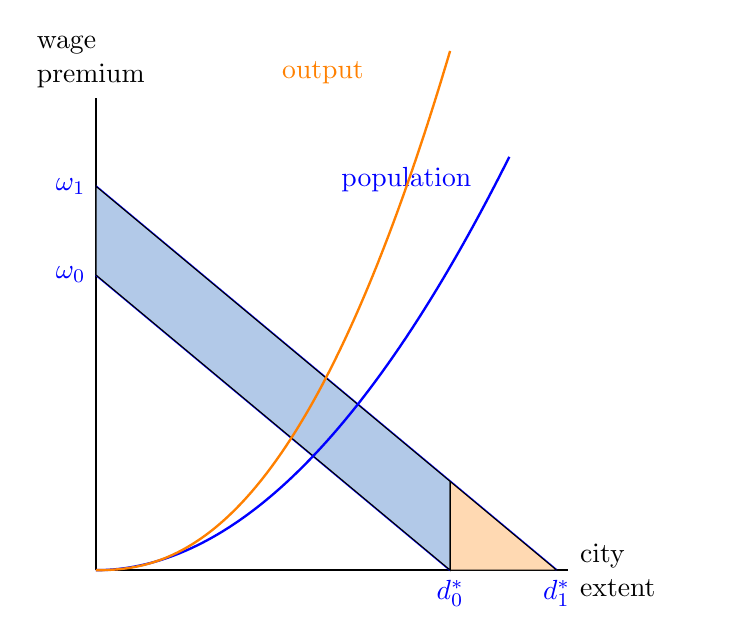
\begin{tikzpicture}[scale=.75]
\def\bndmax{8} 
\tikzset{func/.style={color=blue!80}}	
% EXTENT  BEFORE
\draw[thick](0,0)--(0,8)node[above, text width=1.5cm]{wage \newline premium}; % Y axis
\draw[thick](0,0)--(8,0)node[right=.5, text width=1.5cm]{city\newline extent};  % X axis
%\node at (3.5,-.7){Extent: Walkers};
\draw[thick, blue](0,5)node[left]{$\omega_0$}--(6,0)node[below]{$d^*_0$};
\draw[ thick, blue](0,{5*1.3})node[left]{$\omega_1$}--({6*1.3},0)node[below]{$d^*_1$};
\draw[fill=green!30!blue!30](0,5)--(0,{5*1.3})--(6,5*0.3)--(6,0)--cycle;
\draw[fill=orange!30]({6*1.3},0)--(6,5*0.3)--(6,0)--cycle;
\draw[func, domain=0:7, line width=.3mm,blue, text width=2cm] plot [samples=200] (\x,{\x^2/7})node[below left]{population};
\draw[func,  domain=0:6, line width=.3mm, orange, text width=2cm] plot [samples=200] (\x,{\x^2.3/7})node[below left]{output};
%\node[circle,draw=black, fill=white, inner sep=3pt,minimum size=10pt] (b) at (1,2.5) {1};
\end{tikzpicture}
\end{center}
\caption{ADD A CAPTION}
\label{fig----fix_my_label}
\end{figure}

Assuming that marginal and use per new resident is constant, city size will eventually increase in proportion to the increase in the wage, shown as the distance $d^*_0--d^*_1$. Aggregate rent  further expands by the area shown in orange. Population increases in proportion to the square of the increase in the wage, as illustrated with the blue line.  Output increases super-linearly with population, illustrated by the orange line. 

Adding to the  housing stock is a slow process, introducing potentially complex stock/stock-price dynamics.

The increase in population will eventually generate additional agglomeration benefits, further increasing wages. At the aggregate level, this positive feedback appears to be solidly supported, but locally, within firms and between firms there will be long and variable lags. Analytical equilibrium models seek to bypass these messy processes, while agent-based models attempt to incorporate them.



%will raise the wage, attracting more workers. If they are added in suburbs at the edge of the city (Ricardo's extensive margin) virtually all of the wage premium they receive is dissipated in transportation costs. Closer to the centre,  land rents rise. Owner-occupiers capture the increase as property value appreciation. Tenants are likely to be faced with higher rents.      

%If agglomeration is the source of productivity gains, however, the new workers increase the urban premium, further increasing land values and attracting more workers. 

%The rural population consists of uniformly distributed efficient mix of rural capital producers and workers, all of whom receive $\omega$.%\footnote{This does nothing but fix the price of produced capital in terms of the rural wage.} 

 %Owners of urban firms are  conventional  capitalists, who may earn excess profit if they can capture an unearned surplus from labour.  Any unearned surplus increases the return to urban capital relative to rural capital, resulting in continual expansion of the urban economy. Continuous growth in turn results in continuously rising urban land prices and hence housing costs. We ignore the distributional implications of this feature of the model, and focus instead on the part of value produced by the city that appears as land rent. 
